
\documentclass[times, 10pt,twocolumn]{article}
\usepackage{main}
\usepackage{times}
\usepackage{amsmath}
\usepackage{amssymb}
\usepackage{graphicx}
\graphicspath{{../presentation/figures/}{../experiments/}}

\pagestyle{empty}

\begin{document}

\title{Increasing Reward Quality and Density for Verifiable Rewards\\
       via Master/Novice Divergence}

\author{Ana Carolina Ramos Cunha\\
Technical University of Munich\\
\and
Leonard Evers\\
Technical University of Munich\\
\and
Leonhard Driesch\\
Technical University of Munich\\
}

\maketitle
\thispagestyle{empty}

\begin{abstract}
Reinforcement learning for large language models on verifiable tasks---mathematics,
code, and other domains with binary correctness checks---suffers from reward
sparsity: only the final outcome receives a signal, leaving credit assignment
across long chains of thought unresolved. We investigate a Master/Novice
framework that compares a strong policy to a structurally matched but
capacity-reduced \emph{Novice}, obtained by tensor disentanglement of the
Master's MLP weights, and uses their per-token divergence as a dense reward
proxy. We scale this pipeline from toy matrices through GPT-2 to Qwen3.5 models,
engineer stable disentanglement, and validate Novice quality with MMLU rank
sweeps. On MATH-500 rollouts from Qwen3.5-4B, three progressively sharper
intervention tests find that Master/Novice top-1 disagreement does \emph{not}
identify outcome-critical steps: disagreement positions are only marginally more
locally fragile, and the Novice's specific token choices carry no more leverage
than generic perturbations. Master entropy is at least as predictive. We
conclude that naive divergence-based credit assignment is insufficient, discuss
implications for densifying verifiable rewards, and outline integration into RL.
\end{abstract}


\Section{Introduction}

Large language models (LLMs) trained with reinforcement learning often receive only a sparse, verifiable reward at trajectory end---correct
or incorrect---while intermediate tokens receive no direct feedback. This
\emph{reward sparsity} impedes sample efficiency and credit assignment: the
policy cannot tell which reasoning steps were load-bearing and which were
routine~\cite{cui2025prime}.

Recent work densifies rewards without human step labels by exploiting structure
already present in the task or model. VeRPO uses partial test-case pass rates in
code~\cite{wang2026verpo}; PRIME trains an implicit process reward model online
from outcome labels alone~\cite{cui2025prime}; TIP and related methods identify
high-importance tokens via teacher--student divergence in
distillation~\cite{xu2026tip}; and RLVR studies show that a minority of
high-entropy ``forking'' tokens concentrate most of the learning
signal~\cite{wang2025forking}.

This paper explores a complementary idea: construct a weaker \emph{Novice} from
the same base weights as the \emph{Master} via tensor disentanglement, compare
their action distributions on successful Master rollouts, and upweight tokens
where the Master diverges from the Novice---on the premise that such steps rely
on knowledge the Novice lacks and therefore deserve higher credit. Unlike an
externally trained reward model, the Novice shares architecture and tokenizer
with the Master and
offers a continuous knob (rank fraction) for how weak the comparator should be.

Our contributions are threefold. First, we implement an end-to-end
\texttt{NoviceModel} pipeline---disentangle, save/load, bake to a chosen rank,
and generate---and validate it from MNIST-scale MLPs through Qwen3.5-4B.
Second, we characterize disentanglement hyperparameters and Novice quality via
learning-rate sweeps and MMLU rank sweeps. Third, we run a structured negative
result on the core hypothesis: Master/Novice disagreement is not a useful
per-token or per-step credit signal under greedy decoding on MATH-500, despite a
real but local fragility effect at disagreement positions.


\Section{Related Work}

\SubSection{VeRPO: turning partial success into dense verifiable rewards}

Wang et al.\ propose \textbf{VeRPO} (Verifiable Dense Reward Policy
Optimization)~\cite{wang2026verpo}, an RL framework for code generation that
densifies rewards using only verifiable execution feedback---no external reward
model. Standard pass/fail outcome rewards align with functional correctness but
are sparse: when all rollouts in a group share the same binary outcome, group-based
methods such as GRPO receive zero relative advantage and stall. Learned reward
models offer denser signals but risk misalignment, reward hacking, and high
memory cost.

VeRPO's key observation is that partial test success is already available yet
underused: a generated program may pass some unit tests while failing others.
VeRPO assigns each unit test $u_j$ a difficulty weight $w'_j$ estimated
from pass rates in the current rollout group, down-weighting trivial tests the
policy has mastered and up-weighting challenging ones. The \emph{turn-level}
dense reward at step $t$ is the sum of weights over passed tests:
\begin{equation}
R^{\mathrm{turn}}(\tau_i, t)
= \sum_{j=1}^{|U_x|} w'_j \cdot p^{(j)}_{t,i},
\end{equation}
where $p^{(j)}_{t,i} \in \{0,1\}$ indicates whether turn $t$ in trajectory
$\tau_i$ passes test $u_j$. To anchor local progress to end-to-end correctness,
VeRPO adds a \emph{trajectory-level} outcome reward with length decay:
\begin{equation}
\tilde{R}^{\mathrm{traj}}(\tau_i)
= R^{\mathrm{traj}}(\tau_i)\cdot \gamma^{|\tau_i|},
\end{equation}
where $R^{\mathrm{traj}}(\tau_i) \in \{0,1\}$ is full-suite pass/fail and
$\gamma \in (0,1]$ penalizes long multi-turn trajectories. Turn- and
trajectory-level advantages are computed separately and combined:
\begin{equation}
A(\tau_i, t) = A^{\mathrm{traj}}(\tau_i) + \beta \cdot A^{\mathrm{turn}}(\tau_i, t).
\end{equation}

On Qwen3-8B across HumanEval, BigCodeBench, LiveCodeBench, and Codeforces,
VeRPO consistently outperforms outcome-only GRPO and the RM-based AceCoder
baseline, with up to $+8.83$ pass@1 on Codeforces in multi-turn training while
adding less than $0.02\%$ training time overhead and zero extra GPU memory.
VeRPO also reduces the \emph{degenerate group ratio}---fraction of rollout
groups with identical rewards---from ${\sim}60$--$70\%$ under GRPO to below
$25\%$, substantially improving signal efficiency.

One weakness that VeRPO has, however, is its applicability: for now, it is only useful for code generation. It seems feasible to extend it to other tasks where partial success can be measured, but this has not been done yet. By comparison, our approach would have the appeal of being universally applicable within the realm of LLM-oriented reinforcement learning. Our approach is also more fine-grained: paying attention to individual tokens in a trajectory, as opposed to just differentiating more in the weighting and evaluation of rewards that apply to a whole turn or trajectory.


\SubSection{TIP: token importance in on-policy distillation}

Xu et al.\ introduce \textbf{TIP} (Token Importance in on-Policy
distillation)~\cite{xu2026tip} to identify which tokens carry the most useful
learning signal in on-policy knowledge distillation (OPD). In OPD a student
generates its own rollouts while a stronger teacher provides token-level
supervision; not all positions contribute equally.

TIP organizes tokens along two axes: \textbf{student entropy} $h_t$ and
\textbf{teacher--student divergence} $\delta_t$. Informative tokens fall in two
regions: (1)~high-entropy positions where the student is uncertain, and
(2)~low-entropy but high-divergence positions where the student is
overconfident yet wrong relative to the teacher. Student entropy alone is a
strong first-order proxy---retaining the top 50\% highest-entropy tokens via
entropy-based sampling matches or exceeds full-token training while reducing
peak memory by up to 47\%. However, entropy misses a second important region:
when isolated, low-entropy high-divergence tokens alone---fewer than 10\% of all
tokens---nearly match full-token baselines, showing that overconfident
disagreement carries dense corrective signal invisible to entropy-only rules.

TIP motivates \emph{type-aware} token selection that combines uncertainty and
disagreement, analogous in spirit to our Master/Novice divergence hypothesis
but in a distillation rather than RL setting. Experiments span three
teacher--student pairs (Qwen3, Llama, Qwen2.5) on MATH-500, AIME 2024/2025,
and the DeepPlanning agentic benchmark; training on fewer than 20\% of tokens
(Q3-only) can surpass full-token OPD on long-horizon planning tasks.


\SubSection{Beyond the 80/20 rule: high-entropy minority tokens drive effective reinforcement learning for LLM reasoning}

Wang et al.\ analyze reinforcement learning with verifiable rewards (RLVR)
through token \textbf{entropy patterns}~\cite{wang2025forking}. In chain-of-thought
generation, most tokens are low-entropy (completing linguistic or symbolic
structure), while a minority are high-entropy and act as \emph{forking tokens}
that choose among reasoning paths---words like ``however,'' ``thus,'' or
``suppose'' that branch the derivation.

The paper shows that RLVR largely preserves the base model's entropy layout,
adjusting mainly high-entropy positions while low-entropy tokens stay stable.
Building on this, the authors restrict policy-gradient updates to the top 20\%
highest-entropy tokens (masking the bottom 80\%). Surprisingly, this matches
full-gradient DAPO on Qwen3-8B and \emph{exceeds} it on larger models: $+11.04$
on AIME'25 and $+7.71$ on AIME'24 for Qwen3-32B, and $+4.79$ / $+5.21$ on the
14B model. Training exclusively on the lowest-entropy 80\% instead sharply
degrades performance. The learning signal in RLVR is therefore concentrated in a
sparse set of decisive tokens---a finding that complements model-internal
signals such as Master entropy in our credit-assignment experiments and
suggests that densifying rewards may benefit from targeting high-uncertainty
positions rather than uniform per-token weighting.


\SubSection{PRIME: process reinforcement through implicit rewards}

Cui et al.\ propose \textbf{PRIME} (Process Reinforcement through IMplicit
rEwards)~\cite{cui2025prime}, a framework for dense token-level rewards in
online RL using only outcome labels. The central obstacle to dense process
rewards is scalability: explicit process reward models (PRMs) need expensive
step-level annotation and are vulnerable to reward hacking unless updated
online~\cite{cui2025prime}.

PRIME addresses this with \emph{implicit process rewards}. A causal language
model $\pi_\phi$ is trained as an outcome reward model (ORM) with reward
$r_\phi(y) = \beta \log \frac{\pi_\phi(y)}{\pi_{\mathrm{ref}}(y)}$, then
repurposed at inference to emit per-token process rewards
\begin{equation}
r_\phi(y_t) = \beta \log \frac{\pi_\phi(y_t \mid y_{<t})}{\pi_{\mathrm{ref}}(y_t \mid y_{<t})}.
\end{equation}
Because training uses only binary outcome labels on policy rollouts, the implicit
PRM can be updated online alongside the policy, mitigating distribution shift
without a separate PRM annotation pipeline.

Advantages are computed by summing leave-one-out (RLOO) normalized returns from
process and outcome terms separately:
\begin{equation}
A_t = \underbrace{A_t^{\mathrm{process}}}_{\text{dense}} +
      \underbrace{A^{\mathrm{outcome}}}_{\text{sparse}}.
\end{equation}
Starting from Qwen2.5-Math-7B-Base, PRIME achieves roughly $2.5\times$ sample
efficiency and $6.9\%$ higher outcome training reward than outcome-only RLOO at
matched steps; the resulting Eurus-2-7B-PRIME improves the SFT baseline by
$15.1\%$ on average across math and coding benchmarks while using far less data
than Qwen2.5-Math-7B-Instruct. Online PRM update from the SFT initialization is
critical: offline PRMs degrade under distribution shift.

PRIME differs from our approach in how the dense signal is obtained: it learns
a separate reward head from outcome feedback, whereas we hypothesized that a
fixed capacity-reduced copy of the policy could mark important tokens without
additional training. Our experiments below test whether that hypothesis holds.


\Section{Master/Novice Framework}

\SubSection{Problem setup}

We treat autoregressive generation as a Markov decision process: state $s_t$ is
the prompt plus generated prefix $y_{<t}$, action $a_t$ is the next token, and
reward $R$ is binary verifiable correctness at episode end. The goal is a shaping
function $r_t$ with $\sum_t r_t$ correlating with outcome-critical steps.

The \textbf{Master} is the full-capacity policy $\pi_M$. The \textbf{Novice} is
$\pi_N$ derived from the same checkpoint by truncating disentangled MLP factors
to rank fraction $\rho \in (0,1]$. On a Master rollout $\tau = (y_1,\ldots,y_T)$
that reaches a correct answer, we define per-token divergence
\begin{equation}
\delta_t = D\bigl(\pi_M(\cdot \mid y_{<t}),\, \pi_N(\cdot \mid y_{<t})\bigr).
\end{equation}
Large $\delta_t$ is hypothesized to mark steps where the Master uses reasoning
the Novice cannot reproduce---candidate high-credit positions for RL.


\SubSection{Constructing the Novice via tensor disentanglement}

Following the Master/Novice framework of Till (ongoing work, sebis/TUM), we
replace each decoder MLP \texttt{nn.Linear} with a
\texttt{DisentangledLinear} layer. Disentanglement factorizes a weight matrix
into truncatable components $(Q, U, s, V_h)$ via Riemannian optimization over
orthogonal gauge transformations~\cite{wei2025tensor}. After optimization,
\emph{baking} to rank fraction $\rho$ reconstructs a dense weight matrix
keeping only the top $\rho$ fraction of singular values.

The \texttt{NoviceModel} wrapper owns the full lifecycle: load a base causal LM,
swap MLP linears, run disentanglement, persist factors to disk (monolithic or
sharded checkpoints), bake to any $\rho$ without re-downloading, and delegate
\texttt{generate()} to the underlying \texttt{PreTrainedModel}. This preserves
KV-cache compatibility and allows cheap Novice variants from one disentanglement
run.


\SubSection{Proposed reward shaping}

Given Master rollout $\tau$ with verified success, a natural shaping rule is
\begin{equation}
r_t = \alpha \cdot \tilde{\delta}_t + \mathbb{1}[t{=}T]\cdot R_{\mathrm{outcome}},
\end{equation}
where $\tilde{\delta}_t$ is a normalized divergence (e.g., symmetric KL or
top-1 flip indicator) and $\alpha$ controls density. Before committing to RL
training, we ask a narrower diagnostic question: do positions with
$\mathrm{flip}_t = \mathbb{1}[\arg\max\pi_N \neq y_t]$ actually have higher
\emph{outcome leverage} than matched non-flip positions?


\Section{Implementation and Engineering}

\SubSection{Scaling path}

We validated the pipeline incrementally: toy weight matrices and MNIST-scale
MLPs, a small GPT-2, Qwen3.5-0.8B-Base, and finally Qwen3.5-4B---the model
used for credit-assignment experiments. At each stage we checked that baked
Novices at $\rho{=}1$ match the Master numerically and that lower $\rho$
produces measurable capability gaps.


\SubSection{Disentanglement stability}

Disentanglement is sensitive to learning rate. We swept rates
$\{5{\times}10^{-4}, 10^{-3}, 5{\times}10^{-3}, 7{\times}10^{-3}, 10^{-2},
2{\times}10^{-2}, 5{\times}10^{-2}\}$ on a representative Qwen3.5-0.8B MLP
layer for 200 steps, tracking reconstruction cost and effective rank. Very small
rates converge slowly; rates $\geq 10^{-2}$ diverge (cost increases). A
mid-range rate near $10^{-3}$ minimizes cost while reaching a stable effective
rank (Figure~\ref{fig:lr}).

\begin{figure}[t]
  \centering
  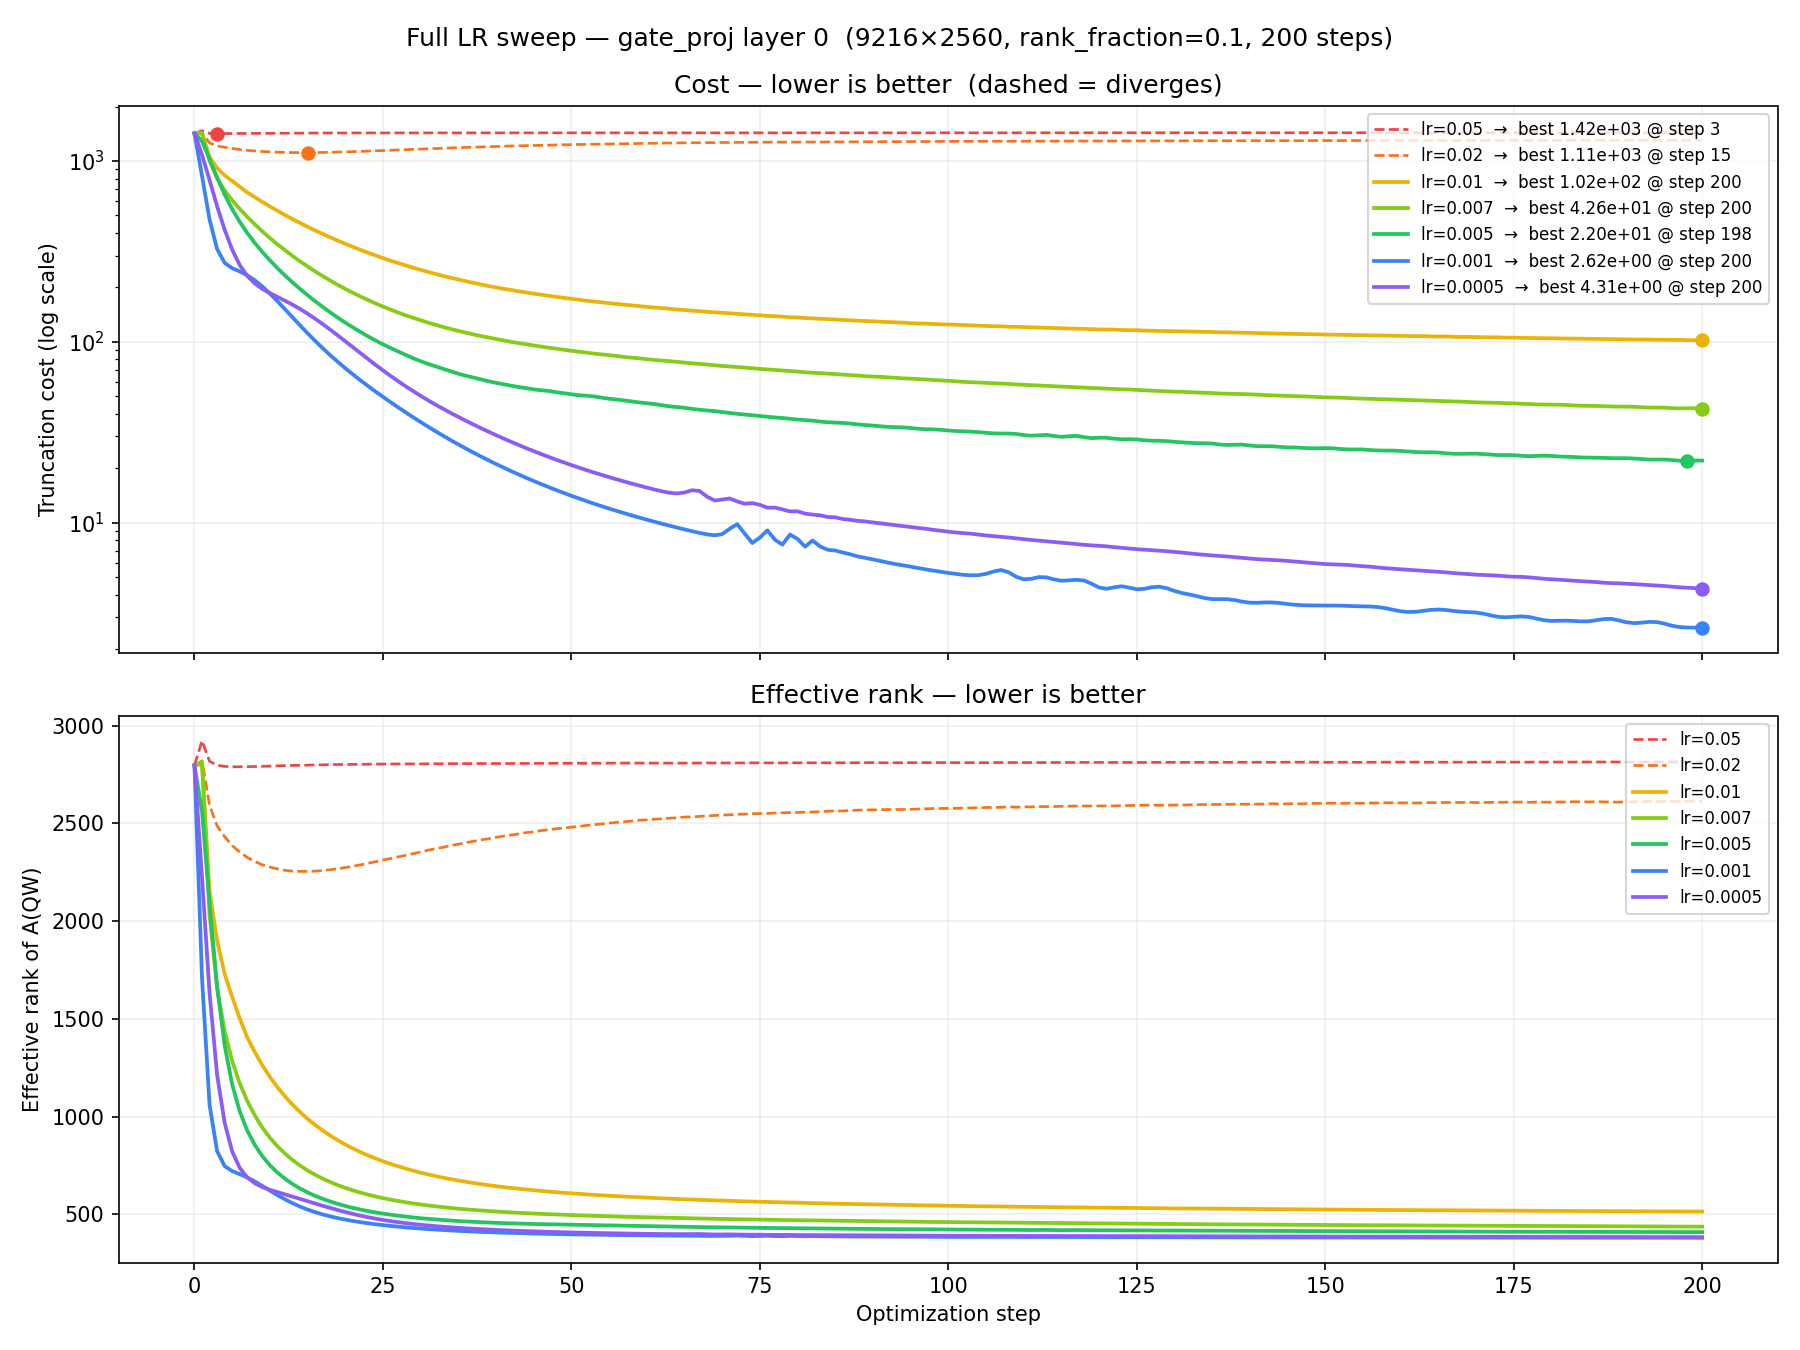
\includegraphics[width=\columnwidth]{figures/lr_sweep.png}
  \caption{Learning-rate sweep for tensor disentanglement. Mid-range rates
    balance convergence speed and stability; large rates diverge.}
  \label{fig:lr}
\end{figure}


\SubSection{Novice quality vs.\ compression}

A useful Novice must be weaker than the Master yet still coherent. On
Qwen3.5-4B, MMLU accuracy stays near the Master down to $\rho \approx 0.5$;
below that, quality drops sharply and the Novice becomes degenerate near
$\rho{=}0.1$ (repetition collapse). This defines a \emph{coherence cliff}: at
$\rho{=}0.1$ roughly 44\% of tokens are top-1 flips, but the Novice's
``disagreements'' are noise; at $\rho{=}0.25$ flips fall to 12\% while the
Novice remains fluent---the sharpest coherent operating point
(Figure~\ref{fig:mmlu}).

\begin{figure}[t]
  \centering
  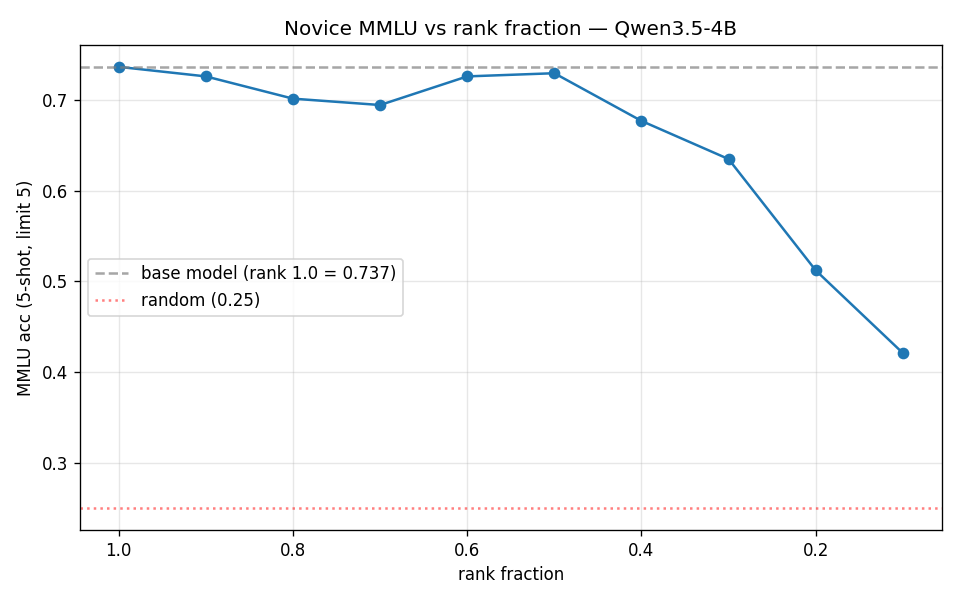
\includegraphics[width=0.85\columnwidth]{figures/mmlu_rank_sweep.png}
  \caption{MMLU accuracy vs.\ Novice rank fraction on Qwen3.5-4B. Accuracy is
    preserved until $\rho \approx 0.5$, then degrades rapidly.}
  \label{fig:mmlu}
\end{figure}


\Section{Credit-Assignment Experiments}

\SubSection{Setup}

\textbf{Models.} Master: \texttt{Qwen/Qwen3.5-4B} (full rank). Novice:
disentangled checkpoint baked at $\rho{=}0.25$.

\textbf{Data.} MATH-500; problems 0--49 with
\texttt{\textbackslash boxed\{\}} instruction. The Master solved 23/50; all
tests use those successful rollouts.

\textbf{Divergence.} Position-aligned \emph{top-1 flip}: Master generates
greedily; Novice is teacher-forced on Master's tokens; a flip at $t$ means
$\arg\max \pi_N(\cdot \mid y_{<t}) \neq y_t$.

\textbf{Grading.} Greedy decoding; pragmatic \texttt{\textbackslash boxed\{\}}
extraction with LaTeX-normalizing equality check.


\SubSection{Experiment 1: release-from-here leverage}

At flip vs.\ depth-matched non-flip position $p$, hand control to the Novice
(prefix $y_{<p}$, then free-run). If flips are pivotal, releasing at a flip
should derail the answer more often.

\textbf{Result} ($n{=}115$ matched pairs): success rate 0.261 (flip) vs.\ 0.270
(control); paired difference $+0.009$. Outcome is governed by release depth,
not flip-ness (108/115 concordant pairs). \textbf{Null.}


\SubSection{Experiment 2: single-token perturbation}

Perturb one token and let the Master continue, isolating causal effect. Arms:
\texttt{flip\_novice} (splice Novice's token), \texttt{flip\_rank2} (Master's
2nd choice at a flip), \texttt{control\_rank2} (Master's 2nd choice at matched
non-flip). Metrics: \emph{local disruption} (drop in log-prob of Master's next 8
tokens), \emph{answer-tied drop}, and free-run binary outcome.

\textbf{Results} ($n{=}345$, 115/arm):
\begin{itemize}
\item Local disruption: flip 2.55 vs.\ control 1.60 nats/tok (gap $+0.94$;
  survives entropy control, $t{=}2.35$)---a modest position signal.
\item Answer-tied drop: null ($t{=}{-}0.14$); magnitudes ${\sim}0.001$ for all arms.
\item Novice's specific token vs.\ generic 2nd choice: null (Novice larger only
  18\% locally, 11\% on answer metric).
\end{itemize}
Local fragility does not propagate to the outcome.


\SubSection{Experiment 3: span (reasoning-step) perturbation}

Perturb a whole newline-delimited reasoning step ranked by flip density; Master
free-runs to the answer. Primary metric: free-run binary correctness.

\textbf{Result} ($n{\approx}50$/arm): flip-dense step break rate 0.151 vs.\ low-
disagreement step 0.176---no gap (if anything, control breaks slightly more).
Novice's version of a step vs.\ generic corruption: identical outcome (0.152 vs.\
0.151). Entropy-controlled answer drop: null ($t{=}{-}0.79$). \textbf{Null} on
the strongest test.


\Section{Discussion}

This work makes concrete progress toward denser verifiable rewards along two
complementary axes: \emph{infrastructure} and \emph{diagnostics}. On the
engineering side, we demonstrated that tensor disentanglement scales from toy
settings to Qwen3.5-4B, that disentanglement hyperparameters can be tuned
reliably, and that Novice quality can be controlled smoothly via rank fraction.
The resulting \texttt{NoviceModel} pipeline---disentangle once, bake to any
$\rho$, and generate on the same architecture as the Master---is a practical
foundation for on-policy comparison without training a separate reward model.

The MMLU rank sweep is particularly encouraging: accuracy remains close to the
Master down to $\rho \approx 0.5$, giving a wide operating range in which the
Novice is meaningfully weaker yet still fluent. Identifying the coherence cliff
and the $\rho{=}0.25$ sweet spot turns an opaque hyperparameter into a usable
design knob. Together with the learning-rate sweep, these results show that
Master/Novice pairs can be produced repeatably at scale, which is a prerequisite
for any downstream reward-shaping method.

Our credit-assignment study then stress-tested the core idea before committing to
full RL training. The three intervention designs---release-from-here, single-token
perturbation, and span-level corruption---form a principled ladder from coarse to
fine causal tests. They establish that simple top-1 flip disagreement is a weak
predictor of \emph{outcome} leverage, while still revealing a genuine local signal
at flip positions and highlighting the Master's striking robustness on MATH-500:
even corrupting whole reasoning steps rarely changes the final answer. That
clarity is valuable: it narrows the search space for viable dense rewards and
motivates richer signals---aggregate divergence mass per trajectory, continuous
divergence measures beyond top-1 flips, or combinations with Master entropy,
which our token-level analysis found to be at least as informative.

Viewed alongside recent dense-reward methods, the Master/Novice framework offers
a distinct and lightweight comparator. PRIME~\cite{cui2025prime} learns implicit
process rewards from outcome labels; VeRPO~\cite{wang2026verpo} exploits partial
test success in code; TIP~\cite{xu2026tip} and high-entropy token
selection~\cite{wang2025forking} identify decisive positions from model-internal
statistics. Our approach does not require additional reward-model training or
task-specific verifiers beyond the outcome check, and it keeps Master and Novice
structurally aligned---properties that remain attractive as we refine \emph{how}
divergence should enter an advantage function. The next natural step is to
integrate the strongest available signals into an RL loop on math reasoning
data and compare sample efficiency against a sparse verifiable baseline.


\Section{Conclusion}

We presented a Master/Novice framework for increasing reward density on
verifiable reasoning tasks. By tensor-disentangling a strong LLM into a
capacity-controlled Novice, we obtain a matched weak policy that can rescore
Master rollouts token by token without leaving the on-policy setting. We
implemented this idea end-to-end in a reusable \texttt{NoviceModel} pipeline,
validated it from small-scale prototypes through Qwen3.5-4B, and characterized
the disentanglement and quality landscape with learning-rate and MMLU rank
sweeps.

On MATH-500, a structured trio of intervention experiments provided a rigorous
read on whether Master/Novice disagreement marks outcome-critical steps. While
naive per-token flip weighting is not supported as a credit signal, the study
delivers actionable guidance: prefer coherent Novices around $\rho{=}0.25$,
expect local but not global effects from disagreement, and consider entropy-aware
or trajectory-level variants when designing dense rewards. These findings
de-risk the path to RL integration and leave us with working infrastructure at
4B scale.

Overall, this project advances the seminar goal of densifying verifiable rewards
by combining a novel comparator-based perspective with reproducible engineering
and careful empirical evaluation. Building on this foundation, we plan to run
Master/Novice rollouts on broader math reasoning benchmarks, explore refined
divergence features, and evaluate whether shaped advantages improve convergence
relative to outcome-only reinforcement learning.
\bibliographystyle{main}
\bibliography{main}

\end{document}
